\documentclass[12pt,a4paper,oneside]{article}

\usepackage[utf8]{inputenc}
\usepackage[english]{babel}
\usepackage{amsmath}
\usepackage{amsfonts}
\usepackage{amssymb}
\usepackage{hyperref}
\usepackage[pdftex,dvipsnames]{xcolor}  % Coloured text etc.
\usepackage{enumerate}% http://ctan.org/pkg/enumerate
\usepackage[separate-uncertainty=true, exponent-product = \cdot, product-units = power]{siunitx}
\sisetup{detect-all}
\usepackage{hyperref}
\hypersetup{
	colorlinks,
	linkcolor = {blue}
}
\usepackage[font=small,format=plain,labelfont=bf,up,textfont=it,up]{caption}


\usepackage{graphicx}
\graphicspath{{./Bilder/}}
\usepackage[left=2cm,right=3cm,top=2cm,bottom=2cm]{geometry}

\usepackage{xargs}                      % Use more than one optional parameter in a new commands
\setlength {\marginparwidth }{2.6cm}
\usepackage[colorinlistoftodos,prependcaption,textsize=tiny,textwidth=\linewidth/1.0]{todonotes}
\newcommandx{\unsure}[2][1=]{\todo[linecolor=red,backgroundcolor=red!25,bordercolor=red,#1]{#2}}
\newcommandx{\abbreviation}[2][1=]{\todo[linecolor=blue,backgroundcolor=blue!25,bordercolor=blue,#1]{#2}}
\newcommandx{\info}[2][1=]{\todo[linecolor=OliveGreen,backgroundcolor=OliveGreen!25,bordercolor=OliveGreen,#1]{#2}}
\newcommandx{\improvement}[2][1=]{\todo[linecolor=Plum,backgroundcolor=Plum!25,bordercolor=Plum,#1]{#2}}
\newcommandx{\thiswillnotshow}[2][1=]{\todo[disable,#1]{#2}}

\newcommand{\fig}{Fig.}
\newcommand{\panda}{\textsc{$\overline{\textsc{P}}$anda}}
\newcommand{\PANDA}{\panda}
\newcommand{\fair}{FAIR}
\newcommand{\btof}{B-ToF}
\newcommand{\btofD}{B-ToF detector}
\newcommand{\SciTil}{\btof}
\newcommand{\btofLong}{Barrel Time-of-Flight Detector}
\newcommand{\btofLongD}{Barrel Time-of-Flight Detektor}
\newcommand{\bdirc}{Barrel DIRC}
\newcommand{\ddirc}{Disc DIRC}
\newcommand{\sm}{Super-Module}
\newcommand{\sensorboard}{Sensor-Board}
\newcommand{\railboard}{Rail-Board}
\newcommand{\hamamatsu}{Hamamatsu}
\newcommand{\ketek}{Ketek}
\newcommand{\advansid}{AdvanSiD}
\newcommand{\antiproton}{anti-proton}
\newcommand{\sipm}{SiPM}
\newcommand{\sipms}{SiPM's}
\newcommand{\proot}{PandaRoot}

\author{Sebastian Zimmermann, Svetlana Chesnevskya}
\title{The Barrel Time-Of-Flight Detector}

\begin{document}

\maketitle

\section*{Aim of the Document}
The aim of this document is to give a broad overview of the detector summarizing and expanding on the established Technical Design Report written by K. Suzuki et al.

\tableofcontents
\newpage

%%%%%%%%%%%%%%%%%%%%%%%%%%%%%%%%%%%%%%%%%%%%%%%%%%%%%%%%%%%%%%%%%%%%%%
\section{Introduction}

The \btofD\ is a scintillating tile hodoscope which used to be referred to as the \emph{SciTil}. It fulfills many functions to support the successful operation of the \panda\ detector. It provides:
\begin{enumerate}[I]
	\item	information for particle identification at low momenta (below the Cherenkov threshold)
	\item	position resolution for track seeding
	\item	timing information to separate individual events in the stream of data
\end{enumerate}


%%%%%%%%%%%%%%%%%%%%%%%%%%%%%%%%%%%%%%%%%%%%%%%%%%%%%%%%%%%%%%%%%%%%%%
\section{The \btof\ Detector Hardware}

The \btofD\ consists of 16 elements arranged symmetrically around the \panda\ interaction point. Each of these elements is called a super-module and comprises four main parts.

\begin{itemize}
	\item Active Medium (Scintillator Tiles)
	\item Photon Readout (\sipm)
	\item Signal Transmission (PCB / \railboard )
	\item Enclosure (Carbon Fiber)
\end{itemize}

A single large PCB or a PCB split into a front and back part connect the Front End Electronics (FEE) to the detector elements. 
Each super-module is equipped with 60 scintillator tiles in two rows, read out by four \sipms\ on each side of the scintillator. 
This adds up to 3840 channels with a total amount of \num{15360} deployed \sipms .

\subsection{Scintillator}
Each scintillator of the \btofD\ is identical to the others and have the following dimensions; \SI{87 x 29.4 x 5}{mm}.
To fit inside the holding structure the corners of the scintillator tiles are truncated.

The scintillator of choice for the detector dimensions is the EJ-232 by Eljen Technology. It is an organic scintillator compound developed for high accuracy timing applications. \todo{add reference or more info}

\subsection{\sipm}

\subsection{\railboard}


%%%%%%%%%%%%%%%%%%%%%%%%%%%%%%%%%%%%%%%%%%%%%%%%%%%%%%%%%%%%%%%%%%%%%%
\section{Infrastructure}

\subsection{Power Supply}

The two main devices that need to be powered are the FEE and the \sipms .
The FEE as they are foreseen at the moment require a \SI{12}{V} supply.
The needs of the \sipms\ depend on the chosen \sipm\ model. Since four \sipms\ are connected in series and the necessary applied voltage adds up, small differences in the operational voltage of individual \sipms\ can change the requirements on the power supply.

In case \hamamatsu\ \sipms\ with an operational voltage of \SI{\sim 60}{V} are used the power supply is required to deliver voltages upwards of \SI{240}{V}.

The TOFPET ASIC system that is foreseen as the base of the FEE is equipped with an internal power supply however only capable of delivering voltages up to around \SI{90}{V}.
As shown this might not be sufficient.
In this case an external power source is required.

The performance of the \sipms\ is also dependant on the applied overvoltage\unsure{does this need explaining?}.
Since the manufacturing of the \sipms\ is not perfect slight variations in the breakdown voltages of every \sipm\ are to be expected.
These variations lead to differences in the applied overvoltage and would need to be adjusted for to ensure identical performance of every detector module, meaning individual power supply channels for every readout channel.
This however is not feasible for the 3840 channels of the detector.

Alternatively multiple detector module can be connected to the same biasing line.
Measurements done in Erlangen with \hamamatsu\ xxx\todo{add sipm model} \sipms\ to determine the optimal bias voltage for each side of the detector showed a slight performance dependance.
If the \sipms\ are pre-sorted and grouped by breakdown voltage the overvoltage mismatch can be minimized.

\subsection{Light Tight Enclosure}

To ensure minimal noise from stray photons the detector super-modules need to be packed in a light tight enclosure.
Similar to the \bdirc\ it is foreseen that the carbon holding frame will act as the photon barrier.

\subsection{Water Cooling of FEE}

The main active component of the \btofD\ is the FEE placed at the end of the detector in front of the interaction point. As the main heat source of the detector it is foreseen to be water cooled.
\todo[inline]{What power draw does the TOFPET ASIC FEB/D have? This needs to be included.}

\subsection{Air Cooling}

Although there is a minimal amount of electrical components placed along the \railboard\ some heat will still be generated; mainly by the \sipms .
Since the \sipm\ performance also is very dependant on the temperature a slight draft of pressured air along the \railboard\ should keep everything dry and produce a constant temperature.

%%%%%%%%%%%%%%%%%%%%%%%%%%%%%%%%%%%%%%%%%%%%%%%%%%%%%%%%%%%%%%%%%%%%%%
\section{Capabilities}

The content of this section is mainly based on work done by Dominik Steinschaden.
For a closer look at the exact methodology behind these concepts and further understanding of the limitations of these processes, the reader is advised to reference The \btof\ TDR (2017) and the dissertation \emph{"Optimization Studies and Performance Simulations for the Time-of-Flight System of PANDA"} (2018)¸ by D. Steinschaden.\unsure{is this relevant?}

The presented capabilities are all based on performance simulations using PandaRoot. The timing based analysis of this detectors data combined with momentum and track information from other detectors allows the \btofD\ to contribute two main features; event building and particle identification.

\subsection{Event Building}

Since \panda\ will not be equipped with a start time detector, the first challenge will be to group relevant hits into single events. This will have to be done before any further analysis of the data stream is possible. For this it is both important to capture all relevant hits and exclude all hits from other events.

For this step the time resolution of the respective detector is the qualifying factor. With average event rates in the high luminosity mode of up to \SI{20}{MHz} or respectively at intervals of of \SI{50}{ns} and individual events at even smaller intervals, an excellent time resolution is required to avoid overlap of relevant detector hits. \fig~\ref{fig:Event_overlap} illustrates the difference a time resolution of \SI{100}{ps} makes compared to a time resolution of \SI{2}{ns}, where hits of multiple events overlap and can not be disentangled.

\begin{figure}
	\centering
	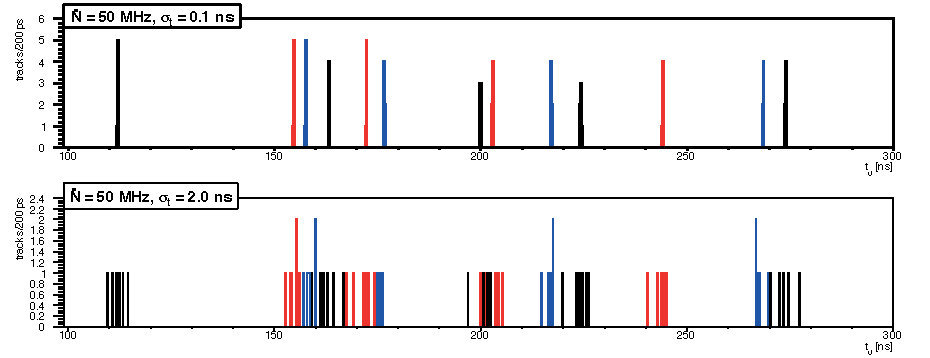
\includegraphics[width = .9\textwidth]{fig/Event_overlap.pdf}
	\caption{Simulation of the hit distribution for an average interaction rate of \SI{50}{MHz} and a detector resolution of \SI{0.1}{ns} and \SI{2}{ns} respectively.}
	\label{fig:Event_overlap}
\end{figure}

\todo[inline]{How exactly this works is in Dominiks Dissertation and needs to be added}

\subsection{Particle Identification and Event Time Determination}

Usually these two tasks are separated and handled by dedicated detectors.
After a start time is determined and a time stamp for a detector hit can be established, the time-of-flight of the respective particle can be calculated.
Combining this information with trajectory length and momentum information provided by the tracking detectors a velocity and hence a mass and particle identity can be determined.
Since \panda\ however has no start time detector, the event time has to be implicitly determined, by combining information of multiple detector hits and various detectors.
The technique used for this is called \emph{Relative Time-of-Flight} and delivers the event time and the respective particle identities of all involved hits simultaneously.

If a hit is registered in the \btofD\ it can not be a very short lived particle due to its radial distance of about \SI{50}{cm} to the interaction point.
This leaves a limited selection of possible particle candidates.
For grouped hits belonging to a single event the procedure is illustrated in \fig ~\ref{fig:relToF}.
Using tracking and momentum information from other detectors, the corresponding interaction time ($t_0$) in the interaction point of every \btof\ hit, can be calculated.
Iterating through all possible mass assumptions produces a distribution of possible $t_0$.
 
\begin{figure}
	\centering
	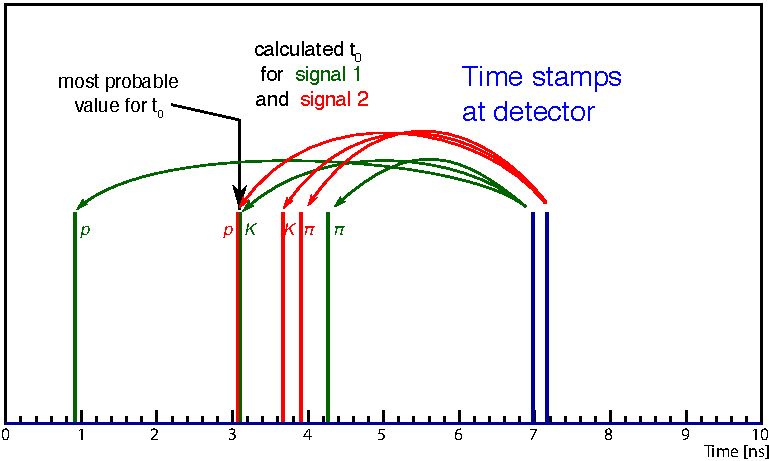
\includegraphics[width=.9\textwidth]{fig/relTof_basic.pdf}
	\caption{The relative time of flight method works by taking multiple mass assumptions of all involved detector hits here marked with blue lines on the time axis. Different
particles show differences in their time-of-flight for the same momentum and trajectory
due to differences in their mass and hence velocity. For these assumptions the respective
interaction or creation time ($t_0$) is calculated and shown color coded; green for the first and
red for the second hit. Where interaction times align we assume to have found $t_0$.}
	\label{fig:relToF}
\end{figure}

Since all hits belong to the same event a cluster of possible $t_0$ values with one candidate from every hit, should emerge.
Taking the mean of these candidate times in the cluster provides us with an estimation of the interaction time, as well as assigning the most likely particle mass to all involved particles.
Thereby identifying the particle species.


%%%%%%%%%%%%%%%%%%%%%%%%%%%%%%%%%%%%%%%%%%%%%%%%%%%%%%%%%%%%%%%%%%%%%%
\section{Performance Validation}

\subsection{Time Resolution Surface Scans}

To ensure a performance as homogeneous as possible over the entire scintillator surface the time resolution was measured at multiple points along the scintillator surface.

These scans were performed at the University of Erlangen in collaboration with the group of A. Lehmann.


%%%%%%%%%%%%%%%%%%%%%%%%%%%%%%%%%%%%%%%%%%%%%%%%%%%%%%%%%%%%%%%%%%%%%%
\section{Calibration}

\subsection{Ongoing Performance Monitoring}

To ensure hardware component issues are detected early the system is supposed to be monitored by small LED's mounted in between the \sipms .
Short bursts of light injected into one side of the scintillator at a time will provide a stable signal source.
Changes in the measured amplitude indicates either an efficiency loss in the scintillator or a gain drop of the involved \sipms .
These signals also act as a reference point in order to determine the time resolution of the detector elements while they are deployed.

It is foreseen to have four channels for all the LED's on one \railboard .
This allows for every other LED on a single side along the board to be illuminated, leaving a dark scintillator between two illuminated scintillators.
This ensures the signal is only produced by the internal light with no light bleed from a neighboring tile.
By only illuminating one side \todo{what is the benefit of this?}

\subsection{Position Calibration}

In order to deliver useful position information for the detector hits the exact position of each tile in the context of the detector needs to be determined.\unsure{this is probably done by in the commissioning phase of the detector setup for the whole experiment.}
The position of the individual scintillator tiles is mainly of interest in the context of the time resolution, signal delay and amplitude drop along the board which are discussed in the following sections.

\subsubsection{Time Resolution Expectancy along the Board}

Since the time resolution is affected by signal noise and decreases of the slope of the rising flank it can be expected to receive a worse time resolution for scintillators farther down the \railboard\ with a longer distance between the detector element and the Front End Electronics.
In order to create a baseline for the detector performance the time resolution needs to be measured along the length of the \railboard .

\subsubsection{Signal Delay along the Board}

In order to provide an accurate time stamp for hits in the \btofD\ the time a signal needs to travel from the \sipms\ to the FEE has to be taken into account. The longer the electrical connection line is the larger the time delay between detector hit and time stamp in the electronics.

The speed a signal travels through a copper connection is significantly slower than the speed of light.

\subsubsection{Amplitude Drop along the Board}


%%%%%%%%%%%%%%%%%%%%%%%%%%%%%%%%%%%%%%%%%%%%%%%%%%%%%%%%%%%%%%%%%%%%%%
\section{Readout}

Foreseen is a readout with the TOFPET ASIC by PETsys Electronics.


\newpage
\listoftodos


















\end{document}
